% Standalone RAKL evidence-maturity traffic light (Paper VI): honest status of evidence classes.
% Build:  pdflatex evidence_maturity.tex  -> evidence_maturity.pdf
\documentclass[border=6pt]{standalone}
\usepackage{tikz}
\usepackage{amsmath}
\usepackage{helvet}\renewcommand{\familydefault}{\sfdefault}
\usetikzlibrary{positioning,arrows.meta,shapes.geometric,fit,backgrounds,calc}
\definecolor{oiblue}{HTML}{0072B2}
\definecolor{oiverm}{HTML}{D55E00}
\definecolor{oigreen}{HTML}{009E73}
\definecolor{oiamber}{HTML}{E69F00}
\begin{document}
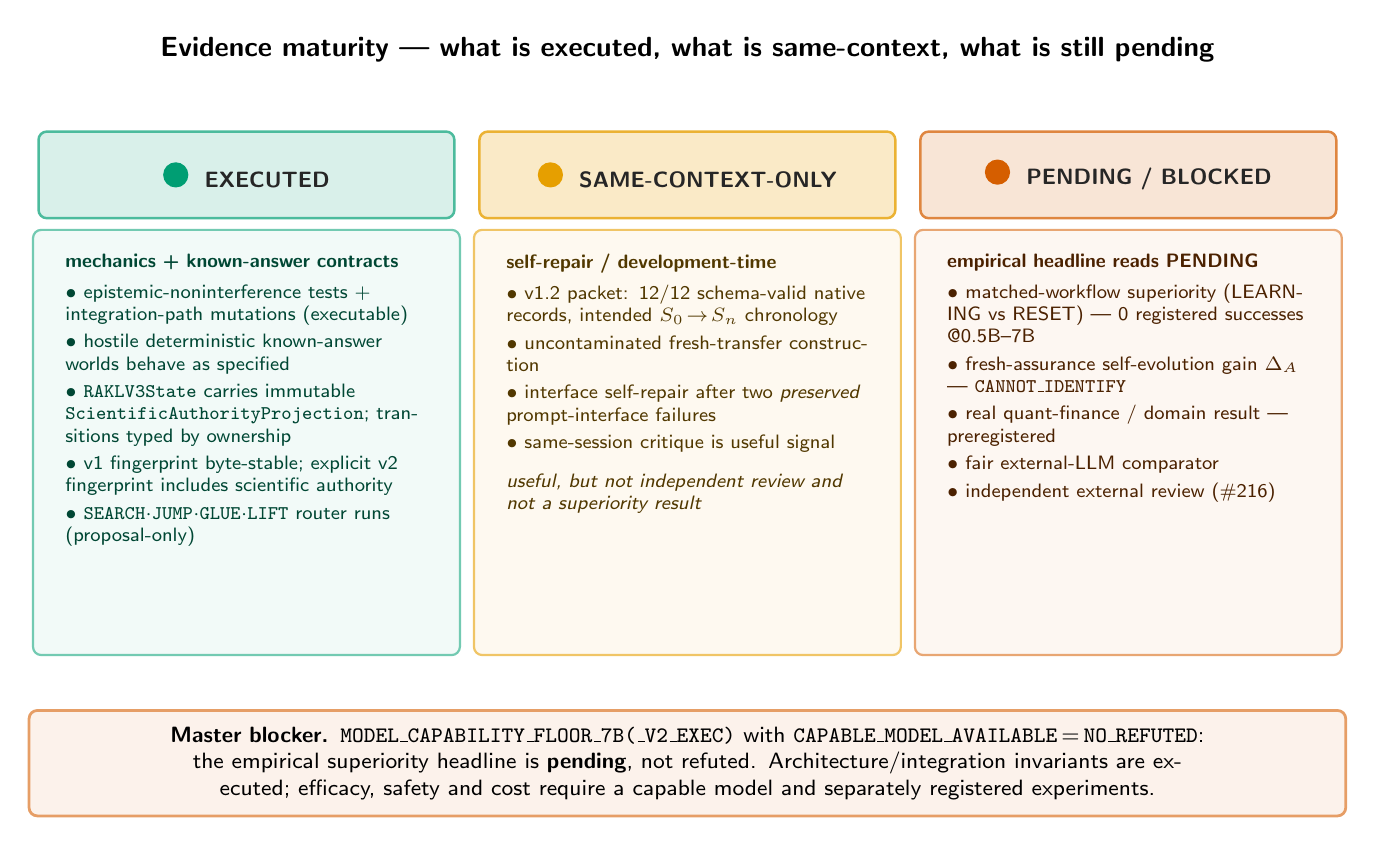
\begin{tikzpicture}[
  font=\small,
  col/.style={rounded corners=3pt, line width=0.8pt, align=center, inner sep=6pt,
              text width=50mm, minimum height=54mm, anchor=north},
  hdr/.style={rounded corners=3pt, line width=0.9pt, align=center, inner sep=4pt,
              text width=50mm, minimum height=11mm, anchor=north, font=\bfseries\footnotesize},
  item/.style={font=\scriptsize, align=left, text width=46mm, anchor=north, text=black!80},
]
\def\cw{5.6}   % column horizontal spacing
% ================= GREEN : EXECUTED =================
\node[hdr, draw=oigreen!70, fill=oigreen!15, text=black!85] (h1) at (0,0)
     {\tikz\fill[oigreen] (0,0) circle (1.6mm); \ EXECUTED};
\node[col, draw=oigreen!55, fill=oigreen!5] (b1) at (0,-1.25) {};
\node[item, text=oigreen!45!black] at ([yshift=-2mm]b1.north)
     {\textbf{mechanics + known-answer contracts}\\[3pt]
      $\bullet$ epistemic-noninterference tests + integration-path mutations (executable)\\[2pt]
      $\bullet$ hostile deterministic known-answer worlds behave as specified\\[2pt]
      $\bullet$ \texttt{RAKLV3State} carries immutable \texttt{ScientificAuthorityProjection}; transitions typed by ownership\\[2pt]
      $\bullet$ v1 fingerprint byte-stable; explicit v2 fingerprint includes scientific authority\\[2pt]
      $\bullet$ \texttt{SEARCH$\cdot$JUMP$\cdot$GLUE$\cdot$LIFT} router runs (proposal-only)};

% ================= AMBER : SAME-CONTEXT-ONLY =================
\node[hdr, draw=oiamber!80, fill=oiamber!22, text=black!85] (h2) at (\cw,0)
     {\tikz\fill[oiamber] (0,0) circle (1.6mm); \ SAME-CONTEXT-ONLY};
\node[col, draw=oiamber!60, fill=oiamber!6] (b2) at (\cw,-1.25) {};
\node[item, text=oiamber!35!black] at ([yshift=-2mm]b2.north)
     {\textbf{self-repair / development-time}\\[3pt]
      $\bullet$ v1.2 packet: 12/12 schema-valid native records, intended $S_0\!\to\!S_n$ chronology\\[2pt]
      $\bullet$ uncontaminated fresh-transfer construction\\[2pt]
      $\bullet$ interface self-repair after two \emph{preserved} prompt-interface failures\\[2pt]
      $\bullet$ same-session critique is useful signal\\[6pt]
      \emph{useful, but not independent review and not a superiority result}};

% ================= GREY/VERMILLION : PENDING / BLOCKED =================
\node[hdr, draw=oiverm!75, fill=oiverm!16, text=black!85] (h3) at (2*\cw,0)
     {\tikz\fill[oiverm] (0,0) circle (1.6mm); \ PENDING / BLOCKED};
\node[col, draw=oiverm!55, fill=oiverm!5] (b3) at (2*\cw,-1.25) {};
\node[item, text=oiverm!35!black] at ([yshift=-2mm]b3.north)
     {\textbf{empirical headline reads PENDING}\\[3pt]
      $\bullet$ matched-workflow superiority (LEARNING vs RESET) --- 0 registered successes @0.5B--7B\\[2pt]
      $\bullet$ fresh-assurance self-evolution gain $\Delta_A$ --- \texttt{CANNOT\_IDENTIFY}\\[2pt]
      $\bullet$ real quant-finance / domain result --- preregistered\\[2pt]
      $\bullet$ fair external-LLM comparator\\[2pt]
      $\bullet$ independent external review (\#216)};

% ================= master blocker banner =================
\begin{scope}[on background layer]
  \node[draw=oiverm!60, line width=1pt, rounded corners=3pt, fill=oiverm!8,
        text width=163mm, align=center, inner sep=6pt, anchor=north,
        font=\footnotesize] (banner) at (\cw,-7.35)
     {\textbf{Master blocker.} \texttt{MODEL\_CAPABILITY\_FLOOR\_7B(\_V2\_EXEC)} with
      \texttt{CAPABLE\_MODEL\_AVAILABLE}\,=\,\texttt{NO\_REFUTED}: the empirical superiority
      headline is \textbf{pending}, not refuted. Architecture/integration invariants are executed;
      efficacy, safety and cost require a capable model and separately registered experiments.};
\end{scope}

% title
\node[anchor=south, font=\bfseries] at (\cw,0.75)
     {Evidence maturity --- what is executed, what is same-context, what is still pending};
\end{tikzpicture}
\end{document}
